\clearpage
%//==============================--@--==============================//%
\subsection[2.2 The Web \& HTTP]{\hspace*{0.075 em}\raisebox{0.2 em}{$\pmb{\drsh}$} The Web \& HTTP}
\label{subsec:the-web-and-http}

\begin{theo}[\underline{World Wide Web (WWW)}]{def:WWW}\label{def:WWW}
    ``The WWW is a global information space that consists of interconnected documents (Web pages) and resources accessible through the internet. The Web is built on top of the \hyperref[def:HTTP]{Hypertext Transfer Protocol (HTTP)}, which is a fundamental protocol used for transmitting and sharing data between web browsers (clients) and web servers.''
\end{theo}

%//==============================--@--==============================//%
\subsubsection[2.2.1 HTTP overview]{$\pmb{\rightarrow}$ HTTP overview}

\begin{theo}[\underline{Hypertext Transfer Protocol (HTTP)}]{def:HTTP}\label{def:HTTP}
    ``HTTP is an application-layer protocol that enables the exchange of documents, images, videos, and other resources on the World Wide Web. It uses a client-server model, where the client initiates requests and the server responds with the requested resource or an error message.''

    \vspace{-0.75em}
    \begin{enumerate}
        \item \textbf{Request-Response Cycle}: Clients (usually web browsers) send HTTP requests to servers, which respond with the requested resource or an error message.
        \item \textbf{HTTP Methods}: HTTP defines several methods, such as \texttt{GET}, \texttt{POST}, \texttt{PUT}, \texttt{DELETE}, and others, to specify the desired action to be performed on the requested resource.
        \item \textbf{HTTP Status Codes}: Servers respond with HTTP status codes to indicate the outcome of an HTTP request. Common status codes include 200 (OK), 404 (Not Found), and 500 (Internal Server Error).
    \end{enumerate}

    \noindent $\pmb{\rightarrow}$ \textbf{Nota:} HTTP utiliza \textbf{TCP} como protocolo de transporte!
\end{theo}

\noindent HTTP é dito um \textit{stateless protocol}, dado que um servidor HTTP n\~ao retem informaç\~ao acerca do utilizador:

\begin{quote}
    ``If a particular client asks for the same object twice in a period of a few seconds, the server does not respond by saying that it just served the object to the client; instead, the server resends the object, as it has completely forgotten what it did earlier.''\cite{Kurose2017}
\end{quote}

\noindent ``HTTP has evolved through several versions, each introducing new features and improvements:
\begin{itemize}
    \item \textbf{HTTP/1.0:} The initial version of HTTP, supporting basic request-response communication and using non-persistent connections.
    \item \textbf{HTTP/1.1:} An updated version that introduced persistent connections, chunked encoding, and improved caching mechanisms.
    \item \textbf{HTTP/2:} A more recent version that offers significant performance improvements, such as multiplexing, header compression, and server push.
    \item \textbf{HTTP/3:} The latest version, currently under development, which aims to improve performance further by using the QUIC transport protocol instead of TCP.'' $[$\textbf{?}$]$
\end{itemize}

%//==============================--@--==============================//%
\subsubsection[2.2.2 Persistência]{$\pmb{\rightarrow}$ Persistência}

\begin{theo}[\underline{Persistência}]{def:Persist}\label{def:Persist}
    ``(...) The application developer needs to make an important decision—should each request/response pair be sent over a separate TCP connection, or should all of the requests and their corresponding responses be sent over the same TCP connection? In the former approach, the application is said to use non-persistent connections; and in the latter approach, persistent connections.''
\end{theo}

\paragraph[2.2.2.1 Sessão não persistente]{$\pmb{\star}$ Sessão não persistente}\mbox{}

\begin{figure}[H]
    \centering
    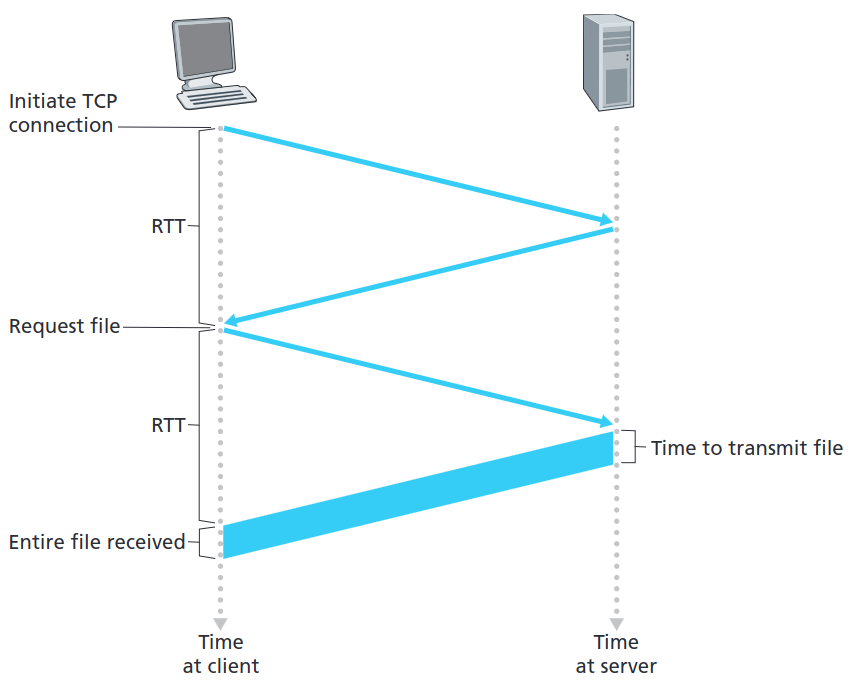
\includegraphics[width = 0.85\linewidth]{img/2/nao-resistente.png}
    \caption{Sessão TCP não persistente}
    \label{fig:nao-persistente}
\end{figure}

\noindent Suponhamos o começo de uma sessão TCP entre um \textit{browser} e um \textit{Web server}. É inicializado o procedimento \textit{three-way handshake}: O cliente (\textit{browser}) envia um pequeno segmento TCP ao servidor, subsequentemente o servidor recebe-o com sucesso e envia de volta um outro segmento TCP. Após completar as primeiras duas partes do \textit{handshake} o cliente envia um pedido HTTP incluindo também a terceira parte do \textit{handshake} (o reconhecimento da receção do segundo segmento). A conexão é solidificada, falta agora atender ao pedido:

\begin{enumerate}
    \item O servidor HTTP busca o objeto de pesquisa, encapsula-o numa mensagem de resposta HTTP e envia-a para o cliente através da \textit{socket}.
    \item O processo servidor indica o termínio da sessão TCP (embora esta não feche até saber o cliente recebeu a mensagem de forma intact).
    \item O cliente recebe a mensagem e consequentemente a sessão TCP é terminada.
\end{enumerate}

\noindent O tempo total de resposta é:
$$
    \boxed{\text{RTT} + \text{RTT} + \text{Time to transmit file}}
$$
\noindent Onde RTT (\textit{round-trip time}) é o tempo que um segmento TCP demora a viajar do cliente ao servidor e viceversa. ``The RTT includes packet-propagation delays, packet-queuing delays in intermediate routers and switches, and packet-processing delays."\cite{Kurose2017}

\vspace{0.6 em}
\noindent\textbf{Nota:} As sessões TCP não persistentes podem decorrer em paralelo, ``most browsers open 5 to 10 parallel TCP connections, and each of these connections handles one request-
response transaction (\textit{forking})"

\paragraph[2.2.2.2 Sessão persistente]{$\pmb{\star}$ Sessão persistente}\mbox{}\\[4pt]
\noindent Na sessões TCP persistentes ocorrem múltiplas transações HTTP por sessão TCP e o servidor não fecha a sessão TCP depois de responder a um pedido. Ocorre canalização (\textit{pipelining}) de pedidos, as respostas são enviadas na ordem de receção:

\vspace{1 em}
\begin{mdframed}
    ``Non-persistent connections in HTTP have limitations, such as the need to establish a new connection for each requested object and a two RTT delivery delay for each object. HTTP 1.1 introduced persistent connections, which allow the server to keep the TCP connection open for multiple requests and responses between the client and server. This enables sending an entire web page or multiple pages from the same server over a single persistent TCP connection. \textbf{Requests can be made back-to-back (pipelining) without waiting for replies to pending requests, and the server typically closes the connection after a configurable timeout interval of inactivity}."
\end{mdframed}

\begin{figure}[H]
    \centering
    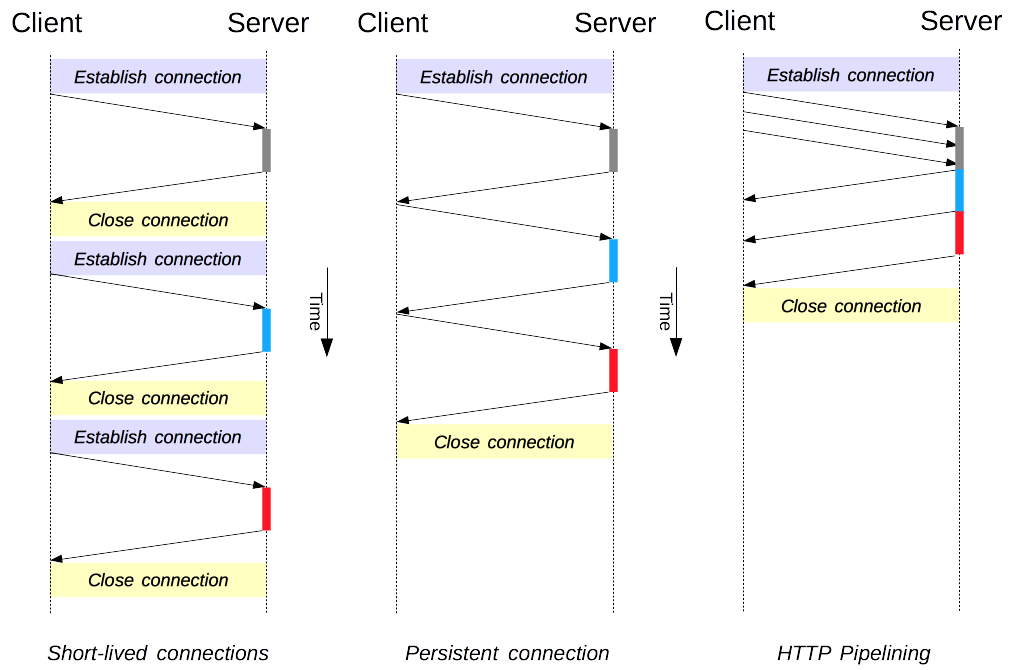
\includegraphics[width = 0.9\linewidth]{img/2/http-connections-example.png}
    \caption{Connection management in HTTP.}
    \label{fig:http-connection-example}
\end{figure}

%//==============================--@--==============================//%
\clearpage
\subsubsection[2.2.3 Transfer-Encoding: chunked]{$\pmb{\rightarrow}$ Transfer-Encoding: chunked}

Chunked encoding is a method used in HTTP to transmit data in smaller, manageable pieces (\textit{chunks}) instead of sending the entire resource in one go.

\vspace{-0.5em}
\begin{enumerate}
    \item \textbf{Purpose:} Enable the server to start transmitting data without knowing the total size of the resource, which is useful for dynamic content generation or when the resource size is unknown in advance.
    \item \textbf{Chunks:} Data is divided into separate chunks, each with its own \underline{size} specified \underline{at the beginning}. The \underline{size is followed by the actual data} and a newline character.
    \item \textbf{Transmission:} The server sends each chunk one by one, with the client assembling the received chunks to reconstruct the original resource.
    \item \textbf{End of data:} A special chunk with a size of zero signals the end of the data transmission, allowing the client to know when it has received the entire resource.
    \item \textbf{Benefits:} Improved responsiveness, as the client can start processing data as soon as the first chunk is received, and reduced resource usage, as the server doesn't need to buffer the entire resource before sending.
\end{enumerate}

\vspace{-0.75em}
\begin{figure}[H]
    \centering
    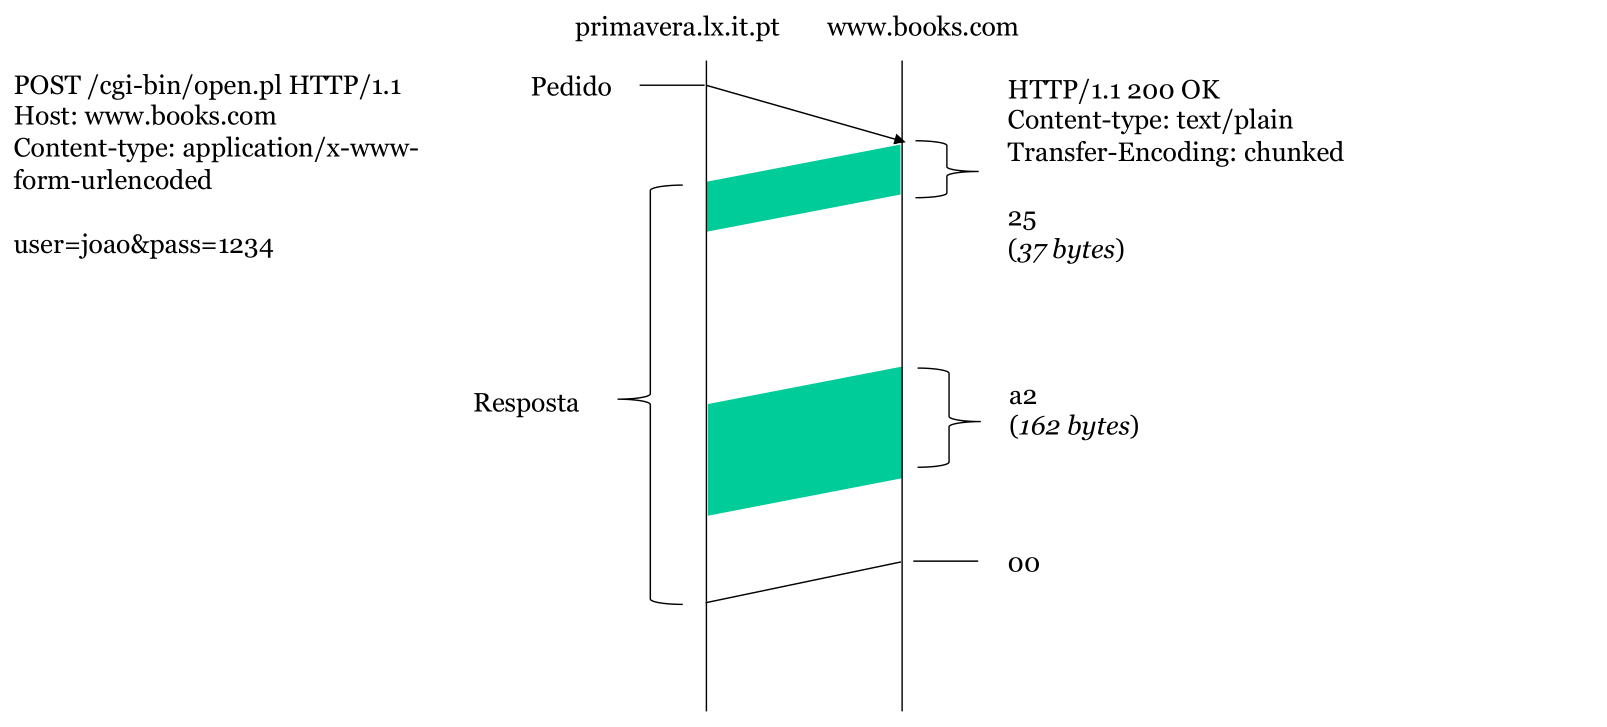
\includegraphics[width = 0.9\linewidth]{img/2/chunked-encoding.png}
    \caption{``Transfer-Encoding: chunked''\protect\cite{slidesSobrinho}}
    \label{fig:chunked-encoding}
\end{figure}

%//==============================--@--==============================//%
\subsubsection[2.2.4 Redirection]{$\pmb{\rightarrow}$ Redirection}

Redirection is a mechanism used in HTTP to inform a client that a requested resource is available at a different URL and instruct it to retrieve the resource from that new location.

\vspace{-0.5em}
\begin{enumerate}
    \item \textbf{Purpose}: Enable web servers to move or rename resources, load balance requests across multiple servers, or enforce URL canonicalization for SEO purposes.
    \item \textbf{HTTP status codes}: Redirection is signaled using HTTP status codes in the 3xx range, with each code indicating a specific type of redirection (e.g., 301 Moved Permanently, 302 Found, 303 See Other, 307 Temporary Redirect).
    \item \textbf{Location header}: The server provides the new URL for the resource in the Location HTTP header of the response. The client should follow the new URL to access the requested resource.
    \item \textbf{Considerations}: Excessive or circular redirections can lead to poor user experience and increased server load. It is essential to use the appropriate status codes and manage redirects properly to avoid such issues.
\end{enumerate}

%//==============================--@--==============================//%
\clearpage
\subsubsection[2.2.5 Formato de mensagens HTTP]{$\pmb{\rightarrow}$ Formato de mensagens HTTP}

HTTP communication relies on a request-response model, where the client initiates a request, and the server sends back a response. This exchange typically consists of four components:
\begin{enumerate}
    \item \textbf{Request/Response Line}
    \item \textbf{Headers:} Provides metadata about the request or response, such as content type, content length, and encoding.
    \item \textbf{Blank Line:} A separator between the headers and the message body.
    \item \textbf{Message Body (optional):} Contains the data being sent in the request or response, such as an HTML document or form data.
\end{enumerate}

\paragraph[2.2.5.1 HTTP request]{$\pmb{\star}$ HTTP request}\mbox{}

\begin{figure}[H]
    \centering
    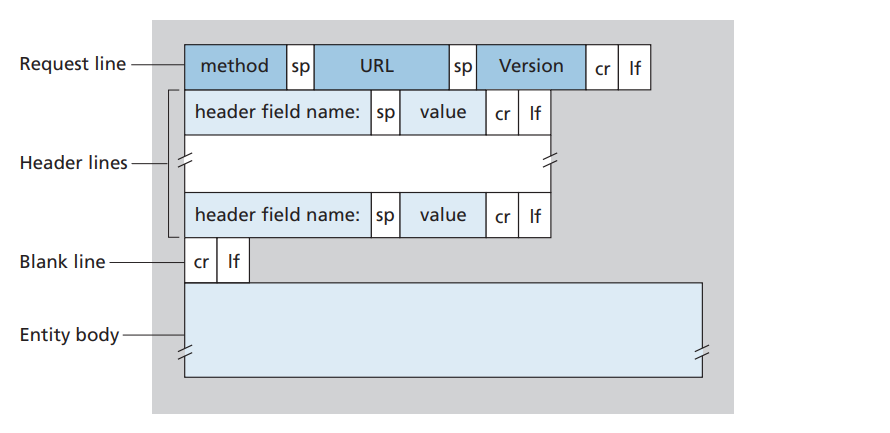
\includegraphics[width = 0.9\linewidth]{img/2/http-request-format.png}
    \caption{``General format of an HTTP request message.''\cite{Kurose2017}}
    \label{fig:http-request-format}
\end{figure}

\noindent HTTP defines several methods (also known as verbs) that indicate the action to be performed on the requested resource. Some of the most common methods include:
\begin{itemize}
    \item \texttt{GET}: Requests data from a specified resource.
    \item \texttt{POST}: Submits data to a specified resource for processing, usually resulting in a change on the server.
    \item \texttt{PUT}: Updates the specified resource with the supplied data.
    \item \texttt{DELETE}: Deletes the specified resource.
    \item \texttt{HEAD}: Similar to \texttt{GET}, but only requests the headers, without the actual data.
    \item \texttt{OPTIONS}: Retrieves the communication options available for the specified resource.
\end{itemize}

\renewcommand*{\thefootnote}{\fnsymbol{footnote}}
\footnotetext[4]{%
A \textit{Uniform Resource Locator (URL)} is a standardized address format used to locate resources on the internet. URLs typically consist of a protocol (e.g., \texttt{http}, \texttt{https}), a domain name or IP address, an optional port number, and a path to the specific resource. For example, \texttt{https://example.com:80/path/to/resource} is a URL, where \texttt{https} is the protocol, \texttt{example.com} is the domain name, \texttt{80} is the port number, and \texttt{/path/to/resource} is the path to the desired resource.
}
\renewcommand*{\thefootnote}{\arabic{footnote}}

\clearpage
\paragraph[2.2.5.2 HTTP response]{$\pmb{\star}$ HTTP response}\mbox{}

\begin{figure}[H]
    \centering
    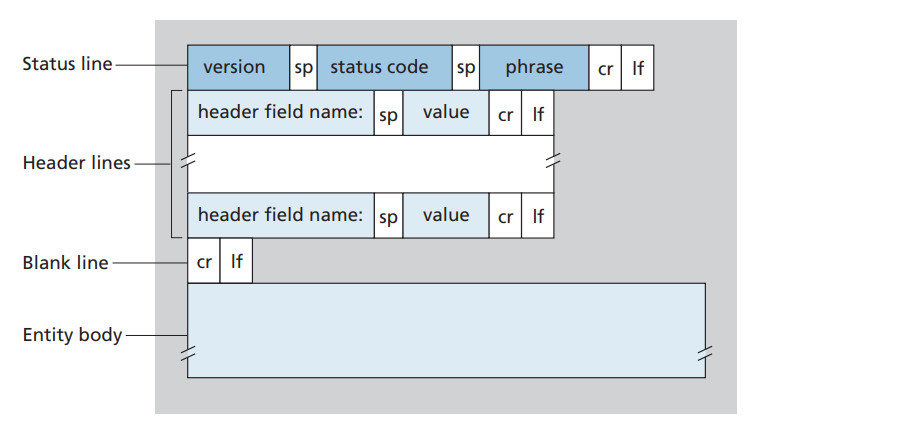
\includegraphics[width = 0.9\linewidth]{img/2/http-response-format.png}
    \caption{``General format of an HTTP response message.''\cite{Kurose2017}}
    \label{fig:http-response-format}
\end{figure}

\noindent HTTP status codes are three-digit numbers included in server responses that indicate the result of the client's request. They are categorized into five classes, based on the first digit:
\begin{itemize}
    \item \textbf{1xx (Informational):} Request received, and the server is continuing to process it.
    \item \textbf{2xx (Successful):} Request successfully received, understood, and accepted.
    \item \textbf{3xx (Redirection):} Request needs further action to be completed, such as following a different URL.
    \item \textbf{4xx (Client Error):} The request contains bad syntax or cannot be fulfilled by the server.
    \item \textbf{5xx (Server Error):} The server failed to fulfill a valid request.
\end{itemize}

%//==============================--@--==============================//%
\subsubsection[2.2.6 Interaç\~ao Cliente-Servidor: \textit{Cookies}]{$\pmb{\rightarrow}$ Interaç\~ao Cliente-Servidor: \textit{Cookies}}

Cookies are small text files stored on a user's device, allowing web applications to remember stateful information across sessions, such as preferences or login data.

\begin{enumerate}
    \item \textbf{Creation:} Servers generate cookies and send them to user's devices via \texttt{Set-Cookie} HTTP headers. The user's web browser then stores the cookie on the device.
    \item \textbf{Cookie usage:} In subsequent requests to the same website, the user's web browser automatically sends the cookie back to the server via the Cookie HTTP header. The server can then use the information in the cookie to customize the user's experience, for example, by displaying a message or remembering items in a shopping cart.
    \item \textbf{Cookie Management:} Websites can update or delete cookies; users can manage them via browser settings.
    \item \textbf{Privacy concerns:} While cookies provide a convenient way to maintain state across multiple sessions, they can also raise privacy concerns due to their ability to track users' browsing habits and collect personal information. Regulations such as the EU's General Data Protection Regulation (GDPR) aim to protect user privacy by requiring websites to obtain user consent before setting cookies and providing options for users to opt-out of tracking.
\end{enumerate}

%//==============================--@--==============================//%
\subsubsection[2.2.7 Web caching]{$\pmb{\rightarrow}$ \textit{Web caching}}

Web cachingis a technique to improve the efficiency and reduce the latency of web access by storing copies of frequently requested resources on a local cache server---also called a \textbf{proxy server}.

\begin{enumerate}
    \item \textbf{Purpose:} Reduce the load on origin servers, decrease network traffic, and improve user experience by providing faster response times.
    \item \textbf{Cache server:} A dedicated server that stores copies of resources, such as images or HTML files, to serve user requests without contacting the origin server.
    \item \textbf{Cache hit:} When a requested resource is found in the cache server, it's called a cache hit. The cache server then serves the resource directly to the user.
    \item \textbf{Cache miss:} When a requested resource is not found in the cache server, it's called a cache miss. The cache server must fetch the resource from the origin server, store it locally, and serve it to the user.
    \item \textbf{Cache replacement:} Due to limited storage capacity, cache servers employ replacement policies (e.g., Least Recently Used) to determine which resources to evict when the cache is full.
    \item \textbf{Conditional \texttt{GET}:} To ensure content freshness, cache servers can issue conditional \texttt{GET} requests, which only retrieve a resource if it has changed since the cache server's last fetch.
    \item \textbf{Collaborative caching:} Cache servers can work together to share resources, reducing redundant downloads and improving overall caching efficiency.
\end{enumerate}

\paragraph[2.2.6.1 Conditional \texttt{GET}]{$\pmb{\star}$ Conditional \texttt{GET}}\mbox{}

\begin{enumerate}
    \item \textbf{\texttt{If-Modified-Since}:} The client includes the \texttt{If-Modified-Since} HTTP header in its request, specifying the date and time of its last request for the resource. The server checks whether the resource has been modified since the specified date and time.
    \item \textbf{Resource status:} If the resource has been modified, the server sends the updated resource along with a 200 OK status code. If the resource has not been modified, the server sends a 304 Not Modified status code without the resource content, indicating that the client's cached version is still valid.
    \item \textbf{\texttt{ETag} and \texttt{If-None-Match}:} An alternative method uses the \texttt{ETag} (Entity Tag) header, which represents a unique identifier for the resource's current version. The client includes the \texttt{If-None-Match} header in its request, containing the \texttt{ETag} value received in the previous response. If the server's current \texttt{ETag} for the resource does not match the value in the \texttt{If-None-Match} header, the server sends the updated resource and its new \texttt{ETag}. If the \texttt{ETags} match, the server responds with a 304 Not Modified status code.
    \item \textbf{Cache validation:} Conditional \texttt{GET} is a crucial component of HTTP caching, as it allows clients to validate their cached resources and refresh them when necessary, without having to download the entire resource each time.
    \item \textbf{Performance benefits:} By reducing the amount of data transferred and allowing clients to reuse cached resources, conditional \texttt{GET} improves network efficiency, reduces server load, and results in faster load times for end users.
\end{enumerate}

%//==============================--@--==============================//%
\clearpage
\subsubsection[2.2.8 HTTP/2: Bloqueio topo-da-fila (\textit{head-of-line blocking})]{$\pmb{\rightarrow}$ HTTP/2: Bloqueio topo-da-fila (\textit{head-of-line blocking})} %adoro-te

\begin{theo}[\underline{Head-of-line blocking (HOL)}]{def:HOL}\label{def:HOL}
    ``Head-of-line blocking (HOL blocking) in computer networking is a performance-limiting phenomenon that occurs when a line of packets is held up in a queue by a first packet.''
\end{theo}

\noindent A versão HTTP/1.1 procura evitar este fenómeno recorrendo à abertura de várias sessões TCP paralelas, permitindo a renderização de objetos mais pequenos e subsequentemente diminuindo o \textit{user-perceived delay}. No entanto, o mecanismo de controlo de congestão inerente ao protocolo TCP força a abertura inadvertida de múltiplas conexões paralelas (exaustando assim as \textit{sockets} do sistema operativo):

\begin{quote}
     ``TCP congestion control inadvertently encourages browsers to use multiple parallel TCP connections instead of a single persistent connection. This is because congestion control aims to distribute an equal share of the available bandwidth to each TCP connection sharing a bottleneck link. By opening multiple parallel connections, a browser can "cheat" and acquire a larger portion of the link bandwidth."\cite{Kurose2017}
\end{quote}

\noindent A versão HTTP/2 procura otimizar o uso da funcionalidade de controlo de congestão bem como reduzir o número de conexões paralelas abertas:

\begin{itemize}
  \item \textbf{Framing e Multiplexagem de streams}: HTTP/2 breaks messages into small frames and interleaves request and response messages on the same TCP connection, significantly reducing user-perceived delay.
  The framing sub-layer of HTTP/2 breaks down HTTP messages into independent frames and reassembles them on the other end. This allows for interleaving and more efficient processing.
  
  \item \textbf{Binary encoding e compressão}: Frames are binary encoded (uma frame para o cabeçalho e outras múltiplas para o corpo da resposta), making them more efficient to parse, slightly smaller, and less error-prone.
  
  \item \textbf{Response message prioritization}: Clients can prioritize responses by assigning a weight between 1 and 256, allowing the server to send higher-priority frames first. Clients can also state each message's dependency on other messages.
  
  \item \textbf{Server pushing}: HTTP/2 enables servers to send multiple responses for a single client request, pushing additional objects to the client without the client having to request each one. This eliminates extra latency due to waiting for requests. (Servidor envia objetos que sabe que o cliente vai precisar sem que este lhe envie os pedidos correspondentes).
\end{itemize}

\begin{figure}[H]
    \centering
    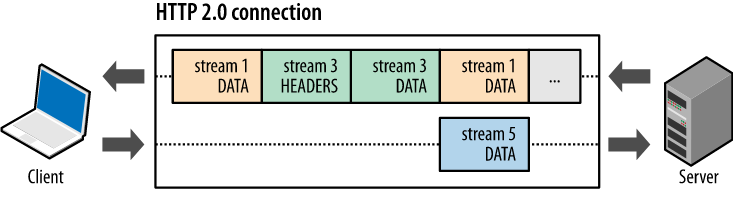
\includegraphics[width = 0.9\linewidth]{img/2/HTTP2.png}
    \caption{Multiplexagem de \textit{streams} de \textit{frames}}
    \label{fig:http2}
\end{figure}